\subsection{Robustness to missing readings and measurement noise}
\label{sec:res-robust}

\Cref{fig:robust} summarises three robustness experiments on unseen stations.

\begin{figure}[t]
  \centering
  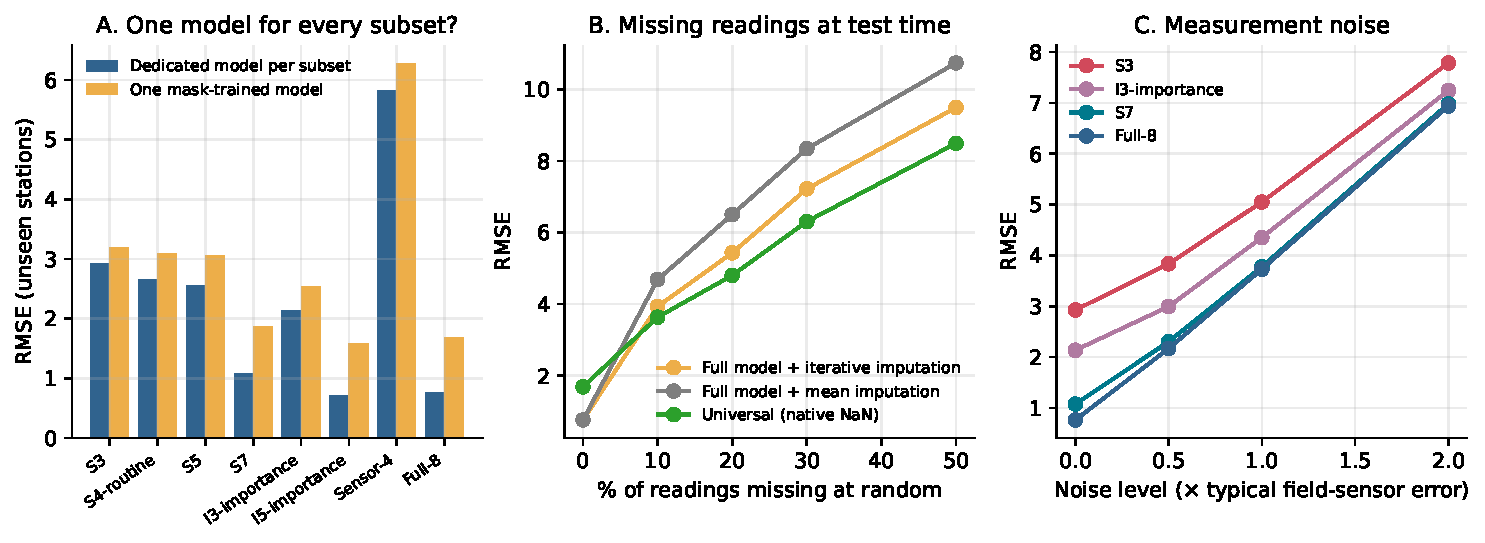
\includegraphics[width=\textwidth]{fig_rob_all.pdf}
  \caption{(A) One mask-trained XGBoost serving every subset versus a dedicated model per subset. (B) Readings missing completely at random at test time. (C) Gaussian measurement noise on test inputs, in multiples of typical field error ($\sigma_{\text{pH}}=0.1$, $\sigma_{\text{DO}}=0.3$\,mg/L, BOD 15\%, turbidity 10\%, nitrate 15\%, EC 5\%, coliforms 50\%).}
  \label{fig:robust}
\end{figure}

\paragraph{(A) One model for all subsets is convenient but costs accuracy.} A single XGBoost trained on randomly masked copies of the data can accept any subset, with missing values as NaN. It is only slightly worse than dedicated models for the small subsets (\sub{S3}: RMSE 3.20 vs 2.93; category accuracy 89.9\% vs 90.6\%). For the large ones it is clearly worse (\sub{Full-8}: 1.69 vs 0.76). Training separate models is cheap, so the recommended deployment is a \emph{bank} of dedicated subset models with routing on the observed parameters. All 255 have already been fitted (\cref{sec:res-subsets}).

\paragraph{(B) Missing readings.} When 10--50\% of the readings in a full-panel visit go missing at random, the mask-trained model with native NaN handling degrades most gracefully. At 30\% missing its RMSE is 6.31, against 7.22 with iterative imputation and 8.34 with mean imputation. Even 10\% random missingness (RMSE 3.6--4.7) is worse than simply using the \sub{S3} model (2.93). The reason is that random missingness sometimes removes pH or BOD, which no imputer can recover. Imputing a missing pH or BOD is worse than routing to a model that never needed it.

\paragraph{(C) Measurement precision matters more than parameter count.} At typical field-instrument noise (scale 1), RMSE rises to 5.05 for \sub{S3}, 4.35 for \sub{I3} and 3.73 for \sub{Full-8}. A noisy full panel is therefore \emph{worse} than a clean three-parameter panel (2.93). Applying noise to one parameter at a time (\cref{tab:noise}) shows that almost all of this comes from \textbf{pH}. An error of only $\sigma=0.1$ pH units raises the \sub{Full-8} RMSE from 0.76 to 3.13, because the pH sub-index changes by 6.7 points per 0.1 pH above 7 and carries 40\% of the weight. BOD at 15\% relative error is the second-largest source. Noise on EC and on the coliforms, even at 50\%, has no effect.

\begin{table}[h]
\centering\small
\caption{RMSE when typical field noise is applied to one parameter at a time (XGBoost, unseen stations; clean RMSE in the first column).}
\label{tab:noise}
\begin{tabular}{lrrrrrrrrr}
\toprule
Subset & clean & pH & BOD & DO & Turb. & Nitrate & EC & Fecal & Total \\
\midrule
\sub{S3} & 2.93 & 4.43 & 3.68 & 3.03 & -- & -- & -- & -- & -- \\
\sub{I3} & 2.14 & 3.75 & 3.13 & -- & 2.17 & -- & -- & -- & -- \\
\sub{S7} & 1.08 & 3.25 & 2.29 & 1.19 & 1.10 & -- & 1.08 & 1.09 & 1.08 \\
\sub{Full-8} & 0.76 & 3.13 & 2.11 & 0.90 & 0.80 & 0.78 & 0.76 & 0.76 & 0.77 \\
\bottomrule
\end{tabular}
\end{table}

\begin{keybox}[Finding 4]
For the CPCB index, a pH reading accurate to $\pm$0.05 is worth more than five extra parameters. A monitoring programme that adopts a reduced panel should invest the savings in pH calibration (two-point buffer calibration before each run) and in BOD quality control.
\end{keybox}

\subsection{Sensitivity to the definition of the index}
\label{sec:res-sens}

\paragraph{(A) Standard values.} We measure how the target changes when each standard $S_i$ is halved or doubled (all weights are recomputed). The index is highly sensitive to the BOD standard: halving it to 1.5 mg/L changes the category of 47\% of visits. It is moderately sensitive to the turbidity and nitrate standards (6--12\% category changes), and insensitive to the coliform and EC standards ($\le$0.3\%). \textbf{Sweeping the EC standard from 250 to 4,000 \si{\micro S/cm} changes the index by at most 0.26 points and the category of at most 0.35\% of visits.} This closes the project's open concern that the EC standard was the least well-sourced value: under CPCB weighting, its value barely matters. The \sub{S3} model remains accurate under every variant (\R{}\,=\,0.90--0.98). It is weakest when the turbidity standard is halved, which doubles the weight of the parameter \sub{S3} cannot see.

\iffull
\begin{figure}[t]
  \centering
  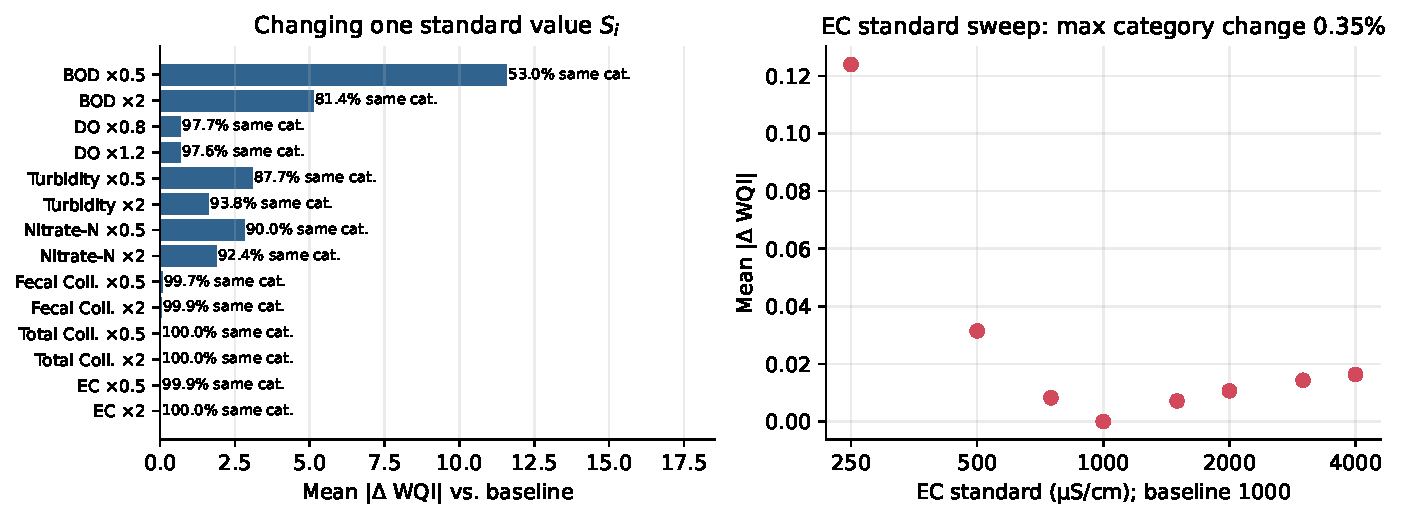
\includegraphics[width=\textwidth]{fig_sens_standards.pdf}
  \caption{Left: mean absolute change of the index, and share of visits keeping their category, when one standard is halved or doubled. Right: EC standard sweep.}
  \label{fig:sensstd}
\end{figure}
\fi

\paragraph{(B) Equal weights reverse the importance ranking.} If every capped sub-index is given equal weight $1/8$, the variance share of the index moves to the parameters the CPCB weights ignore (\cref{fig:senseq}): fecal coliform 27\%, total coliform 25\%, turbidity 18\% and BOD 15\%, with pH only 4\%. The two indices are only moderately rank-correlated ($\rho_S=0.74$). Under this target \sub{S3} collapses to \R{}\,=\,0.62 (rank 47 of 56), and \sub{I3} to 0.80. The best three-parameter subset becomes turbidity, EC and total coliform (0.91). Only \sub{S7} is near the top under \emph{both} definitions (0.994 and 0.990), because it contains BOD, turbidity and both coliforms.

\begin{figure}[t]
  \centering
  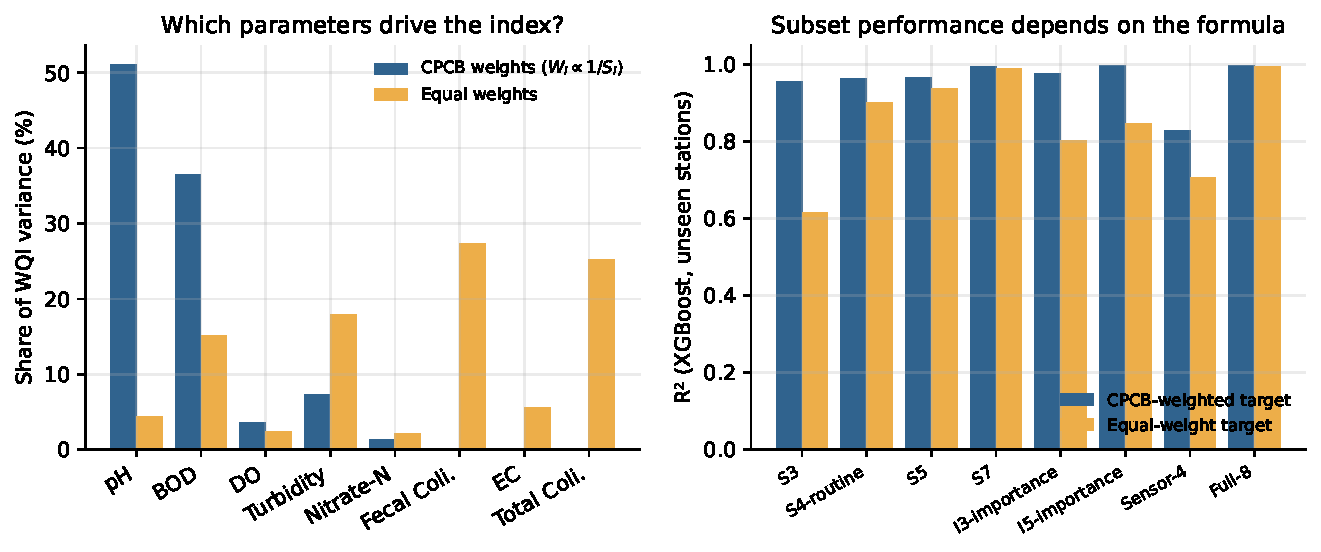
\includegraphics[width=\textwidth]{fig_sens_equalweight.pdf}
  \caption{Left: variance share per parameter under CPCB and equal weights. Right: station-held-out \R{} of the named subsets for the two targets.}
  \label{fig:senseq}
\end{figure}

\paragraph{(C) Uncapped index.} Predicting the uncapped index (on a $\log_{10}$ scale, five categories including ``Unsuitable'') is a different problem. Its extreme values are driven by turbidity spikes and occasional BOD spikes. \sub{S3} reaches only \R{}\,=\,0.37 and recalls 54\% of Unsuitable visits. Adding turbidity changes everything: \sub{I3} reaches 0.98 with 94\% Unsuitable recall, and \sub{S7} 0.993 with 97\% (\cref{tab:uncapped}).

\begin{table}[h]
\centering\small
\caption{Predicting the uncapped index (XGBoost on $\log_{10}$ WQI, unseen stations).}
\label{tab:uncapped}
\begin{tabular}{lrrrr}
\toprule
Subset & \R{} ($\log$) & 5-class acc. & Unsuitable recall & Median rel.\ error \\
\midrule
\sub{S3} & 0.374 & 45.6\% & 53.5\% & 27.4\% \\
\sub{S4-routine} & 0.631 & 62.9\% & 72.6\% & 16.0\% \\
\sub{S5} & 0.698 & 65.2\% & 73.1\% & 14.6\% \\
\sub{I3-importance} & 0.980 & 90.5\% & 94.3\% & 3.7\% \\
\sub{Sensor-4} & 0.925 & 77.8\% & 87.3\% & 8.1\% \\
\sub{S7} & 0.993 & 95.3\% & 97.4\% & 1.7\% \\
\sub{Full-8} & 0.994 & 96.1\% & 97.6\% & 1.6\% \\
\bottomrule
\end{tabular}
\end{table}

\begin{keybox}[Finding 5]
\emph{Which} reduced panel is adequate depends on the index definition. pH + BOD (+DO) suffices for the capped CPCB index. Detecting extreme events (the uncapped index) requires turbidity, and an index that gives bacteria real weight requires the coliforms. \sub{S7} is the only subset that is robust across all three definitions.
\end{keybox}

\subsection{Deployment: reconstructing WQI where it was never computed}
\label{sec:res-deploy}

\paragraph{Scope.} 20,132 river visits report pH, DO and BOD but not the full panel: 5,337 in 2018, 5,705 in 2019, 2,240 in 2020 and 6,850 in 2021. They come from 819 stations on 70 rivers. \textbf{255 of these stations never had a single full-panel visit}, so they have never had a WQI. 16,686 of the visits also report fecal coliform and can use \sub{S4-routine}.

\paragraph{Covariate shift.} The deployment visits are distinguishable from the labelled ones: an adversarial classifier on (pH, DO, BOD) reaches AUC 0.77. The shift is mostly in BOD (KS $=0.25$--$0.31$; median 2.2--2.5 vs 1.7 mg/L), and pH, DO and fecal coliform shift only slightly (KS $\le 0.17$)\optref{fig:shift}. Inspecting the raw files shows the cause. \textbf{In 2018, 2019 and 2021 no river visit reports a BOD value at or below 1\,mg/L}, against 22\% of visits in 2020, and 26--28\% of biological rows in those years have a blank BOD (4\% in 2020). The most likely explanation is that below-detection-limit BOD values were left blank in those years. The deployment set is therefore missing its cleanest visits. Fewer than 2\% of deployment values fall outside the 0.5--99.5\% range of the training data, so the model is interpolating, not extrapolating.

\iffull
\begin{figure}[t]
  \centering
  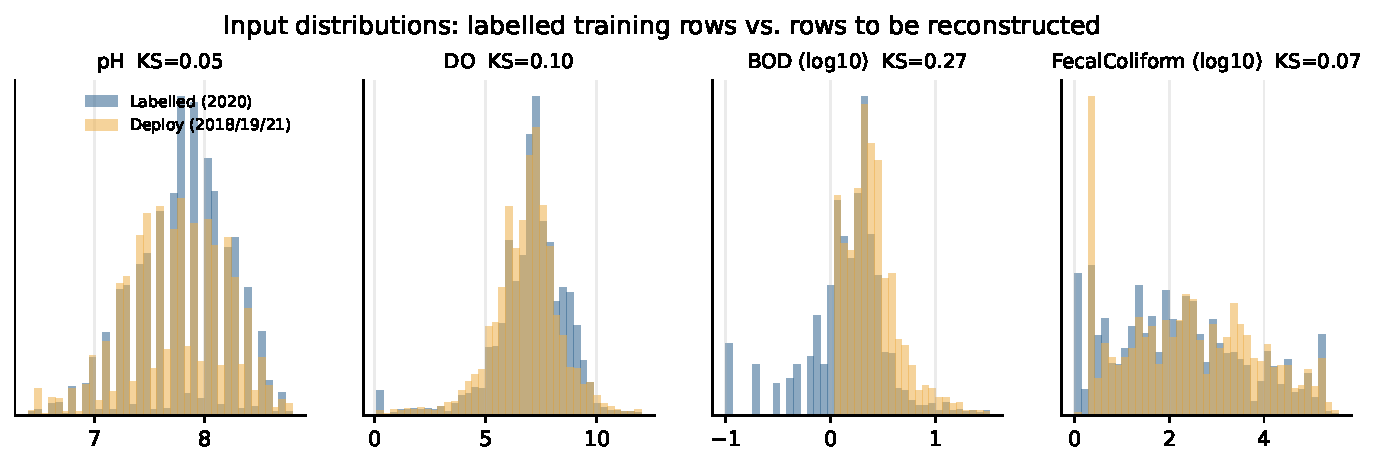
\includegraphics[width=\textwidth]{fig_dep_shift.pdf}
  \caption{Inputs of labelled (2020) versus deployment (2018/2019/2021) visits. Note the absence of BOD $\le$ 1\,mg/L ($\log_{10}\le 0$) in the deployment years.}
  \label{fig:shift}
\end{figure}
\fi

\paragraph{Expected error under the shift.} The station-CV errors are re-weighted by the density ratio $p(\text{deploy}\mid x)/p(\text{labelled}\mid x)$ from the adversarial classifier (effective sample size 2,107). This estimates the expected error on the deployment distribution: \sub{S3} RMSE \textbf{3.01} (unweighted 2.93), category accuracy 90.0\% (90.6\%), and 90\% conformal-interval coverage 88.3\% (90.0\%). For \sub{S4-routine} the figures are 2.75, 91.3\% and 89.1\%. The shift therefore costs little accuracy. Restricted to labelled visits with BOD $>1$, the \sub{S3} error is unchanged (RMSE 2.89).

\paragraph{Results.} \Cref{fig:depyear} shows the reconstructed index by year. Mean predicted WQI is 63.0 (2018), 62.3 (2019), 54.7 (2020, unlabelled visits) and 60.9 (2021), against a true 2020 mean of 56.1. The apparent ``2020 was cleaner'' effect is almost entirely the BOD reporting floor. Restricted to BOD $>1$\,mg/L, the true 2020 mean is 60.3 and the predicted 2020 mean 59.4, in line with the other years. Year-to-year comparisons must therefore condition on BOD $>1$, or treat the blanks as left-censored values, before they are interpreted as trends.

\begin{figure}[t]
  \centering
  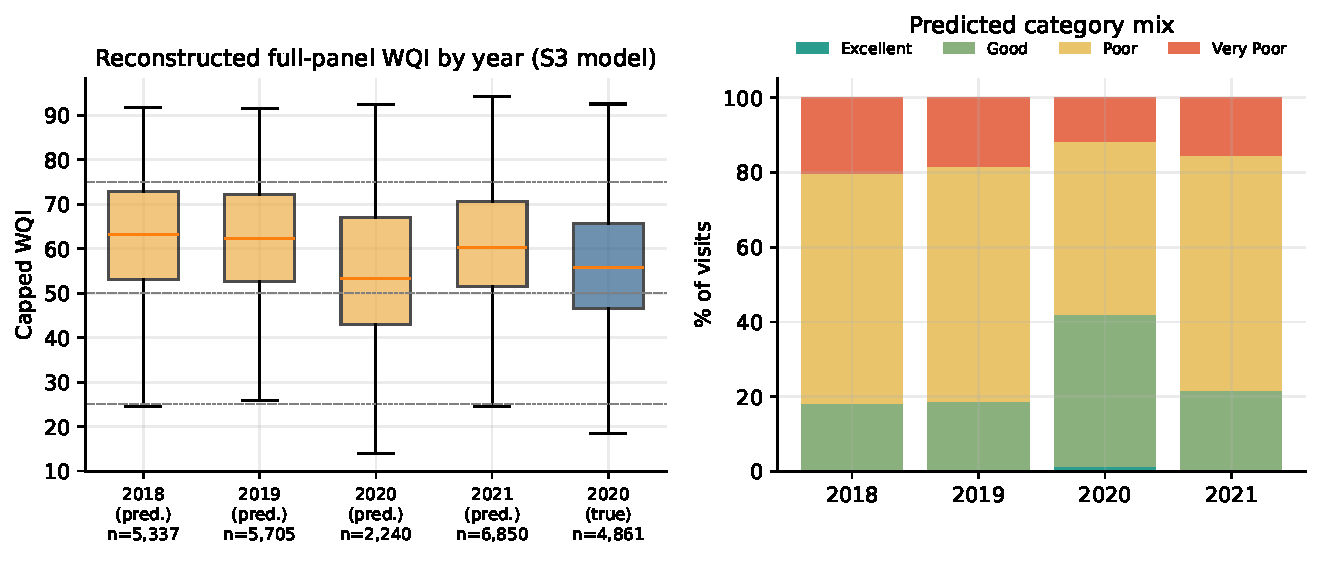
\includegraphics[width=\textwidth]{fig_dep_by_year.pdf}
  \caption{Reconstructed full-panel WQI (\sub{S3} model) for visits without a full panel, by year, against the true 2020 labelled values. Right: predicted category mix.}
  \label{fig:depyear}
\end{figure}

The \sub{S3} and \sub{S4-routine} reconstructions agree closely (correlation 0.994, mean absolute difference 1.2 points). The station ranking is persistent across years: the correlation between a station's true 2020 mean and its reconstructed mean in another year is 0.60 (2018), 0.71 (2019), 0.73 (2021) and 0.80 (2020, other visits). The river-level reconstruction\optref{fig:depriver} is consistent with known conditions. The Gomti and Bhima are worst in every year, and the Brahmani, Narmada and Mahanadi are consistently in the better half, as in the 2020 ground truth. The renormalised formula would have reported these visits 3.5 points worse on average than the model. \iffull\Cref{fig:depmap} maps the reconstructed index, including the 255 stations that gain a WQI for the first time.\fi

\iffull
\begin{figure}[t]
  \centering
  \begin{subfigure}[t]{0.52\textwidth}
    \centering
    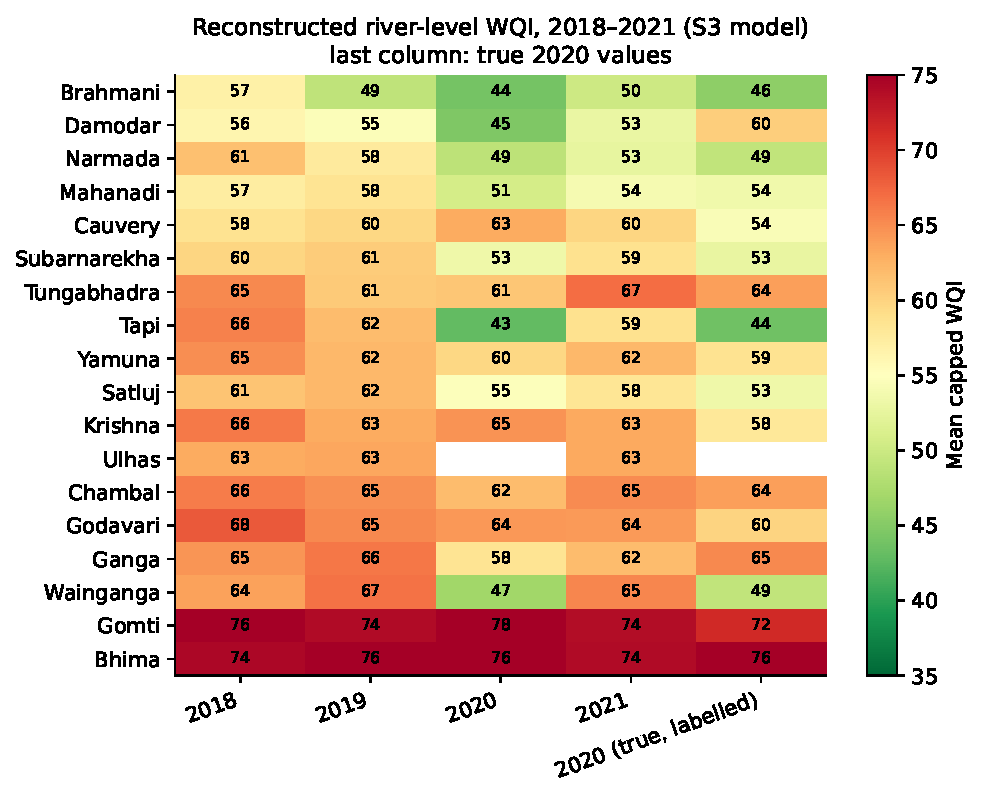
\includegraphics[width=\textwidth]{fig_dep_river_year.pdf}
    \caption{River $\times$ year (18 largest rivers).}
    \label{fig:depriver}
  \end{subfigure}\hfill
  \begin{subfigure}[t]{0.46\textwidth}
    \centering
    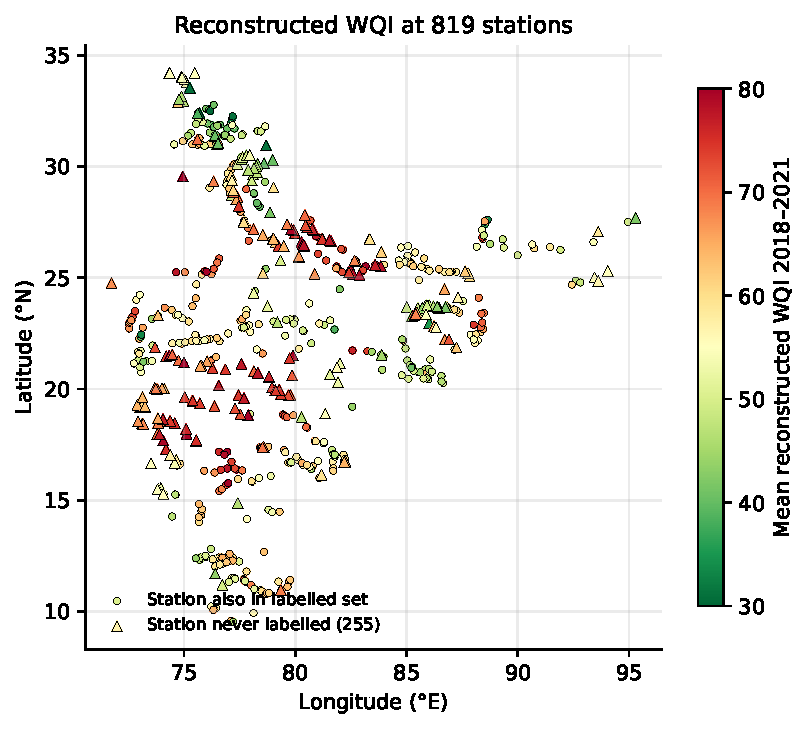
\includegraphics[width=\textwidth]{fig_dep_map.pdf}
    \caption{Station means, 2018--2021.}
    \label{fig:depmap}
  \end{subfigure}
  \caption{Reconstructed WQI. In (b), triangles mark stations that never had a full-panel WQI.}
\end{figure}
\fi
